\documentclass{ltjsarticle}
%%%package読み込み
\usepackage{amsmath}
\usepackage{amssymb}
\usepackage{amsfonts}
\usepackage{mathtools}
\usepackage{bm}
% \usepackage{tikz} % ★消去: 代わりに graphicx 追加
% \usetikzlibrary{cd}
\usepackage{url}
\usepackage{graphicx} % ★追加: 図を挿入するため
\usepackage{float} % ★追加: 図の位置を制御するため
\usepackage{caption} % ★追加: 図のキャプションを柔軟に扱うため
%\usepackage{xcolor}
\usepackage{ascmac}
\usepackage{tcolorbox}
%\usepackage[dvipdfmx, setpagesize=false, bookmarks=true, bookmarksdepth=tocdepth, bookmarksnumbered=true, colorlinks=true, linkcolor=red]
\usepackage{hyperref}
\usepackage[version=4]{mhchem}
\usepackage{braket} % 追加した
\usepackage{booktabs}
\usepackage{bookmark}
%\usepackage[textwidth=45zw,lines=44]{geometry}
%\usepackage{pxjahyper}
%%%黒板太字
\newcommand{\N}{\mathbb{N}}
\newcommand{\Z}{\mathbb{Z}}
\newcommand{\Q}{\mathbb{Q}}
\newcommand{\R}{\mathbb{R}}
\newcommand{\C}{\mathbb{C}}
\newcommand{\F}{\mathbb{F}}
%%%約物
\newcommand{\abs}[1]{\left|#1\right|}
\newcommand{\lr}[1]{\left(#1\right)}
\newcommand{\st}{\; \mathrm{s.t.}\; }
\newcommand{\Ae}{\textrm{-a.e.}} 
%%%繰り返し
\newcommand{\pluss}[3]{#1_{#2}+\cdots+#1_{#3}}
\newcommand{\minuss}[3]{#1_{#2}-\cdots-#1_{#3}}
\newcommand{\timess}[3]{#1_{#2}\times\cdots\times #1_{#3}}
\newcommand{\leqs}[3]{#1_{#2}\leq\cdots\leq #1_{#3}}
\newcommand{\geqs}[3]{#1_{#2}\geq\cdots\geq #1_{#3}}
\newcommand{\opluss}[3]{#1_{#2}\oplus\cdots\oplus #1_{#3}}
\newcommand{\otimess}[3]{#1_{#2}\otimes\cdots\otimes #1_{#3}}
\newcommand{\commas}[3]{#1_{#2},\ldots,#1_{#3}}
%%%微分
\newcommand{\dx}[1]{\mathrm{d}#1}
\newcommand{\ddx}[1]{\frac{\mathrm{d}}{\mathrm{d}#1}}
\newcommand{\dydx}[2]{\frac{\mathrm{d}#1}{\mathrm{d}#2}}
\newcommand{\dydxn}[3]{\frac{\mathrm{d}^{#3}#1}{\mathrm{d}#2^{#3}}}
\newcommand{\del}[2]{\frac{\partial#1}{\partial#2}}
\newcommand{\dell}[2]{\frac{\partial^2#1}{{\partial#2}^2}}
\newcommand{\deln}[3]{\frac{\partial^{#3}#1}{{\partial#2}^{#3}}}
%%%
%%%演算子
%log type
\let\Re\relax
\DeclareMathOperator{\Re}{Re}
\let\Im\relax
\DeclareMathOperator{\Im}{Im}
\DeclareMathOperator{\sgn}{sgn}
\DeclareMathOperator{\sign}{sign}
\DeclareMathOperator{\Supp}{Supp}
\DeclareMathOperator{\tr}{tr}
\DeclareMathOperator{\Tr}{Tr}
\DeclareMathOperator{\Det}{Det}
\DeclareMathOperator{\Log}{Log}
\DeclareMathOperator{\rank}{rank}
\DeclareMathOperator{\diag}{diag}
\DeclareMathOperator{\corank}{corank}
\DeclareMathOperator{\Res}{Res}
\DeclareMathOperator{\Ker}{Ker}
\DeclareMathOperator{\coker}{coker}
\DeclareMathOperator{\Coker}{Coker}
\DeclareMathOperator{\Var}{Var}
\DeclareMathOperator{\Cov}{Cov}
\DeclareMathOperator{\sech}{sech}
\DeclareMathOperator{\csch}{csch}
\DeclareMathOperator{\arcsec}{arcsec}
\DeclareMathOperator{\arccot}{arccot}
\DeclareMathOperator{\arccsc}{arccsc}
\DeclareMathOperator{\arccosh}{arccosh}
\DeclareMathOperator{\arcsinh}{arcsinh}
\DeclareMathOperator{\arctanh}{arctanh}
\DeclareMathOperator{\arcsech}{arcsech}
\DeclareMathOperator{\arccsch}{arccsch}
\DeclareMathOperator{\arccoth}{arccoth}
\DeclareMathOperator{\grad}{grad}
\let\div\relax
\DeclareMathOperator{\div}{div}
\DeclareMathOperator{\rot}{rot}
%\DeclareMathOperator{\GL}{GL} % ★消去 : ここから↓
%\DeclareMathOperator{\SL}{SL}
%\DeclareMathOperator{\Sym}{Sym}
%\DeclareMathOperator{\Aut}{Aut}
%\DeclareMathOperator{\Inn}{Inn}
%\DeclareMathOperator{\Out}{Out}
%\DeclareMathOperator{\id}{id}
%\DeclareMathOperator{\pr}{pr}
%\DeclareMathOperator{\supp}{supp}
%\DeclareMathOperator{\diam}{diam}
%\DeclareMathOperator{\End}{End}
%\DeclareMathOperator{\Cl}{Cl}
%\DeclareMathOperator{\Hom}{Hom} % ★消去 : ここまで↑
%limit type
\DeclareMathOperator*{\argmin}{arg~min}
\DeclareMathOperator*{\argmax}{arg~max}
%%%
%%%定理
\usepackage{amsthm}
\theoremstyle{definition}
\newtheorem{lem}{補題}
\newtheorem*{lem*}{補題}
\newtheorem{prf}{証明}
\newtheorem*{prf*}{証明}
\newtheorem*{ex*}{Example}
\newtheorem*{rem*}{Remark}
\newenvironment{prb}[1]%
{\begin{itembox}[l]{\textbf{問題 #1}}}%
{\end{itembox}}
\newenvironment{sol}[2]%
{\setcounter{lem}{0}
\setcounter{prf}{0}
\par\noindent\textbf{解答 #1} (#2)\par}%
{\par\normalfont}

\renewcommand{\refname}{Reference}


%%%%%%%%%%%%%%%%%%%%%
\numberwithin{equation}{section}
%%%%%%%%%%%%%%%%%%%%%%

\newcounter{boxeddefcounter}
\newenvironment{problem}
{\refstepcounter{boxeddefcounter}\begin{itembox}[l]{問\theboxeddefcounter}}
{\end{itembox}}

%\usepackage[hang,small,bf]{caption}
%\usepackage[subrefformat=parens]{subcaption}
\captionsetup{compatibility=false}


\newcommand{\D}{^\circ\text{C}}
\newcommand{\ka}{\textasciitilde}


\pagestyle{myheadings}
\title{有機化学実験 文献調査}
\date{\today}
\author{Author: No.7 05253011 Fumiya Kashiwai / 柏井史哉}
\begin{document}
\maketitle
\markboth{Organic experiment Literature report No.7 05253011 Fumiya Kashiwai / 柏井史哉} {Organic experiment Literature report No.7 05253011 Fumiya Kashiwai / 柏井史哉}
%%ここまでタイトル

\newpage
\section{3,6-dymethylphthalic anhydrideの合成}
\subsection{Purpose and Background}
\begin{figure}[htbp]
\begin{center}
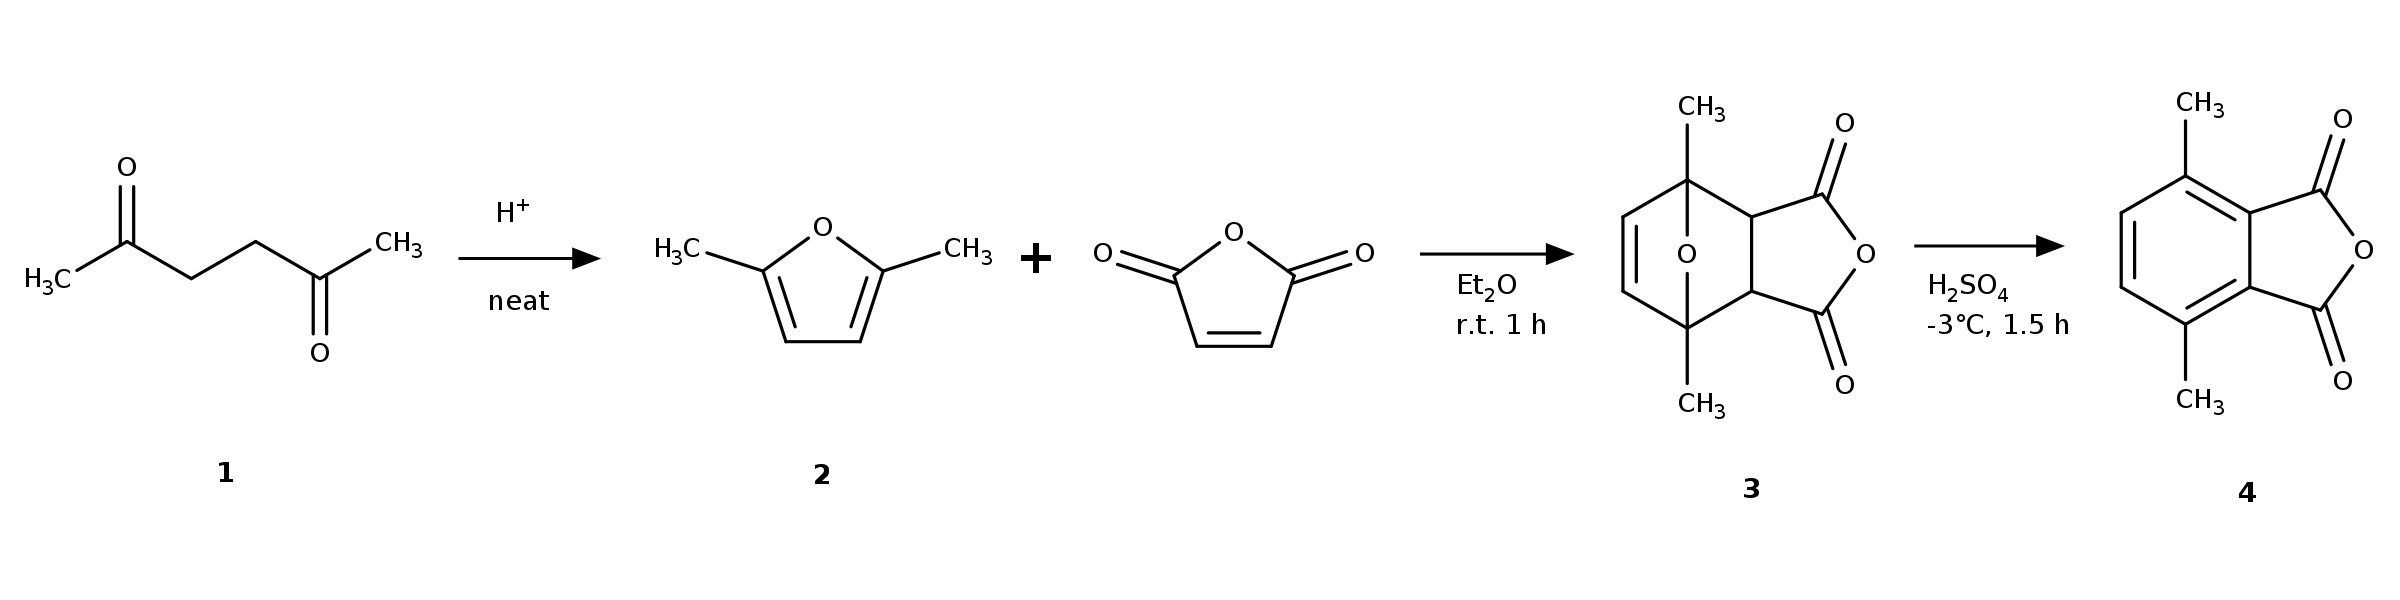
\includegraphics[width = 15 cm]{scheme6-1.png}
\caption{化合物\textbf{4}の合成スキーム}
\label{scheme_6-1}
\end{center}
\end{figure}

\subsection{Experimental}
\begin{enumerate}
\item ナスフラスコにアンバーリスト320 mg、化合物\textbf{1} 21.17 gをとり、マグネティックスターラーで撹拌しながら$130\D$のオイルバスで蒸留して留分を得た。留分は氷冷した。
\item 受けに用いていたフラスコが転倒し、産物をロスしたためあらためて操作を行った。
\item ナスフラスコにアンバーリスト220 mg、化合物\textbf{1} 21.00 gをとり、スターラーで撹拌しながら$130\D$のオイルバスで蒸留して留分を得た。留分は氷冷して得た。
蒸気温度が$75\D$で流出が開始し、蒸気温度が$82\D$まで上昇したのち、$76\D$程度まで低下し液体の流出が穏やかになったところで蒸留を停止した。
\item 得られた留分は下層 (透明) と、上層 (黄色) にほぼ同体積で分離していた。下の水層をピペットで大方取り除いたのち、無水\ce{Na2SO4}を加えて乾燥、ひだつきろしにより濾過することにより化合物\textbf{2}の粗精製物 (9.93 g, 56\%) を得た。
\item 三角フラスコに乳鉢で粉砕した無水マレイン酸 8.09 g、\ce{Et2O} 6 mLを加え、マグネティックスターラーで激しく撹拌して懸濁させた。
\item 化合物\textbf{2}の粗精製物 9.70 gをフラスコに加え、アルミホイルで蓋をして、室温で撹拌したところ、黄色の均質な溶液となった。45 min程度撹拌を続けると白濁し、白色の沈澱が生じた。
\item 生じた沈澱を吸引濾過すると黄色がかった固体を得た。氷冷した\ce{Et2O}で洗浄し、白色の固体\textbf{3} (8.17 g, 48\%) を得た。この固体を風乾し、IR、\ce{^1H NMR}スペクトルを測定した。また、この物質の融点の測定値は$71-72\D$ (文献値: $67-71\D$) であった。
\item 乾燥した三角フラスコに濃\ce{H2SO4} 40 mLをはかりとり、食塩を加えた氷浴により$-6\D$程度に冷却した。温度をモニターしながら、溶液の温度を$-3\D$前後に保って固体\textbf{3} 4.01 gを少しずつ加えた。1 h程度で固体を加え終わったのち、10 min撹拌して溶液が均質になった。
\item 氷浴を外して溶液を室温に戻したのち、300 mLの氷水にゆっくりと加えたところ、白濁した。
\item 吸引濾過ののち、水10 mLで洗浄し粘土状の白色固体を得た。
\item 得られた固体を$10\%$ \ce{NaOH}\textit{aq.} 30 mLに溶かし、\ce{AcOH} 5 mLを加えた。析出した固体をひだ付き濾紙を通して、取り除いた。
\item 濾液に濃塩酸4 mLを加えると白色の結晶が生じた。この結晶を吸引濾過によりろ別した。時間の都合上、結晶の状態で4 days風乾した。
\item 得られた固体をtoluene 50 mLに溶解し、常圧蒸留を行った。はじめ蒸気温度$80\D$程度の成分が流出し、蒸気温度が低下したところで一旦加熱を停止し、熱時濾過により固体を除去した。
\item さらに蒸留を行い、蒸気温度$102\D$程度の成分を得た。全量5 mL程度まで濃縮し、氷冷して無色透明な固体 (0.95 g, 26\%) を得た。得られた固体のIRスペクトル、\ce{^1H NMR}スペクトルを取得した。測定した融点は$145-146\D$ (文献値: $146-147\D$) であった。
\end{enumerate}

\subsection{Result and Discussion}

%推定される反応機構の図

図\ref{mechanism_6-1}に示した反応機構で進行すると推測される。酸触媒下での反応であり、分子間および分子内アルドール反応と目的の反応が競合すると予測される。しかしながら、アルドール反応は可逆であり、目的の反応は脱水を伴うため基本的には不可逆である。そのため最終生成物としては化合物\textbf{2}が優先的に生成すると考えられる。
その後、無水マレイン酸と化合物\textbf{2}の間でDiels-Alder (DA) 反応が生じる。求ジエン\textbf{2}は電子豊富、無水マレイン酸は電子不足であり、このDA反応は良好に進行すると期待される。実際、今回の実験では室温で45 minで完了したと考えられる。その後、硫酸溶媒下で脱水反応を起こして化合物\textbf{4}を得る。\textbf{3}→\textbf{4}の反応は脱水反応であり、生じた水は溶媒の硫酸との溶媒和で熱を生じる。加えて、\textbf{3}→\textbf{4}では芳香環が形成されるため、大きく安定化すると予測され、この反応は非常に発熱的であると期待される。実際、この反応は食塩を加えた氷浴により冷却しながら行ったが、化合物\textbf{3}の粉末を飯能溶液に加えると溶液温度の上昇が見られた。

化合物\textbf{4}の粗精製物に含まれると考えられる副生成物としては、未反応の化合物\textbf{3}および、化合物\textbf{3}、\textbf{4}が加水分解されたジカルボン酸が挙げられる。
精製では、水で希釈した時に析出した固体を塩基性溶液に溶かし、弱酸性にした時に析出した固体を除いたのちに、強酸性にして白色の結晶を得た。化合物\textbf{4}は強酸性条件では水に溶解しない (白色固体として析出する) が、弱酸性-塩基性溶液には溶解していた。この性質を用いることで、他の弱酸性溶液での不純物をまず除くことができると期待される。また、化合物\textbf{4}は芳香環を有するため、tolueneへの溶解性が良いと期待される。対して化合物\textbf{3}は溶解性が悪いと考えられ、toluene溶液の熱時濾過により除去できると考えられる。toluene溶液の蒸留では、最初に$80\D$程度の留分が流出した。tolueneと水は$85\D$で共沸する\cite{solvent_bp}ことから、これにより水を除くことができたと考えられる。その後は$102\D$の留分としてtoluene (沸点$110.6\D$) が得られ、残渣を冷却すると\textbf{4}が析出した。\ce{^1H NMR}スペクトル (fig.\ref{NMR_6-1-3}) では不純物は観測されず、純度よく精製できたと考えられる。
\subsection{Conclusion}

\section{3-methyl-3-(\textit{p-}tolylsulfonyl)-cyclopentanone の合成}
\subsection{Purpose and Background}
\begin{figure}[htbp]
\begin{center}
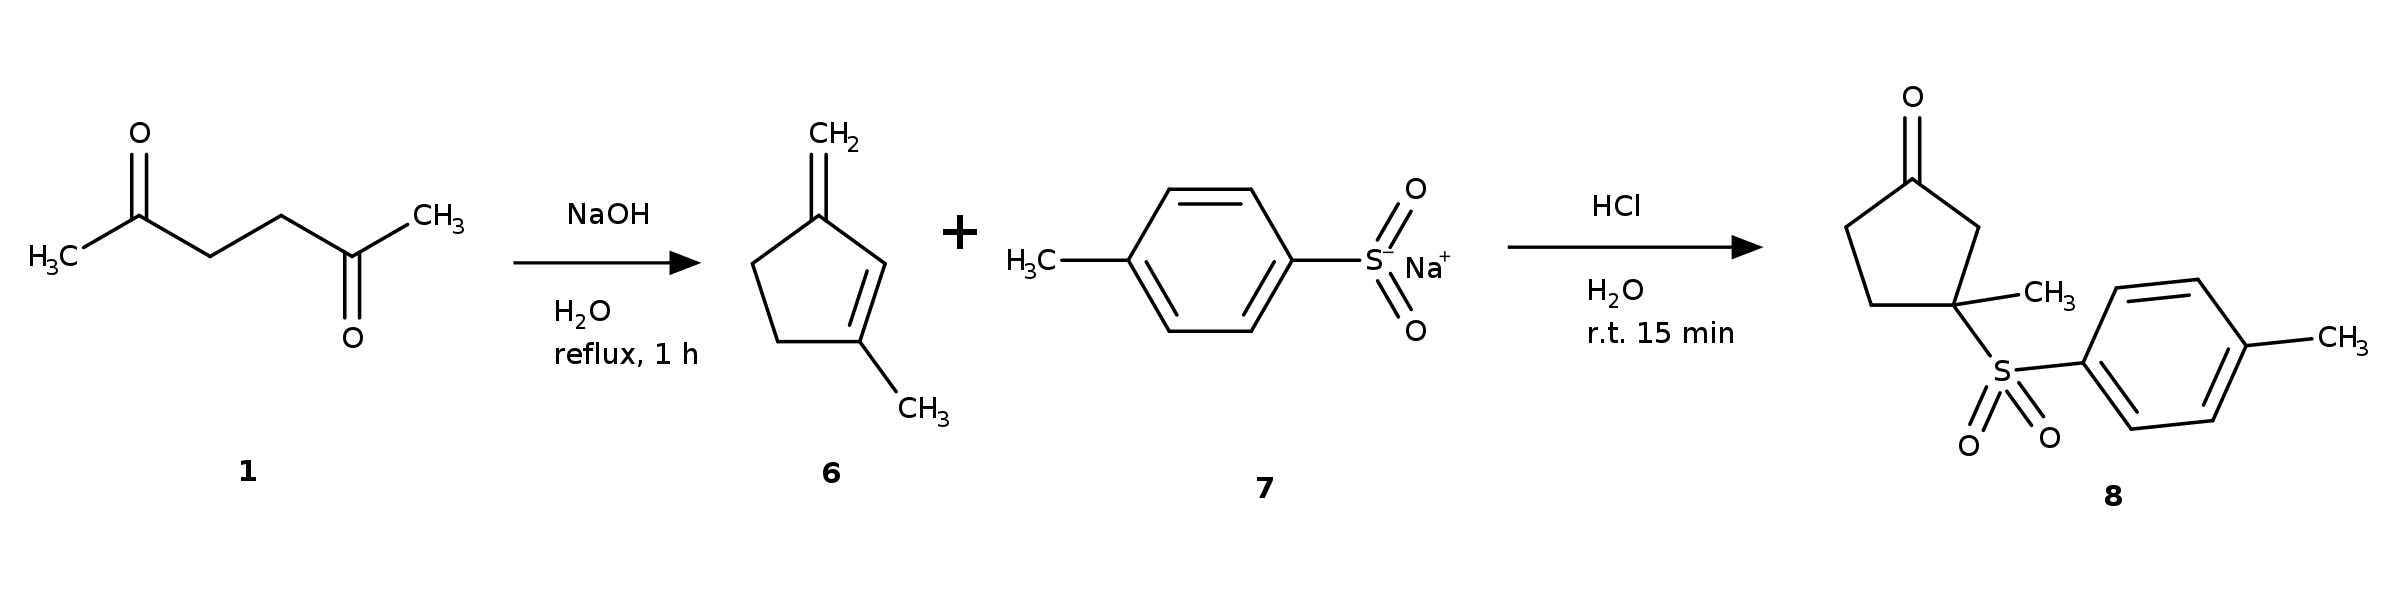
\includegraphics[width = 15 cm]{scheme6-2.png}
\caption{default}
\label{default}
\end{center}
\end{figure}

\subsection{Experimental}
\begin{enumerate}
\item ミツ口フラスコに\ce{NaOH} 1.15 g、水 100 mLを加え、撹拌して均一な溶液とした。
\item 湯浴で$120\D$に加熱し、穏やかに還流させながら滴下管から化合物\textbf{1} 12.60 gを5 minかけて滴下した。 
\item TLCにより反応の進行をモニターし、20 min後に出発物 ($R_f = %
$) の消失確認した。滴下終了後30 min撹拌し、反応を終了とした。
\item 氷冷により室温まで冷却したのち、\ce{NaCl} 10.56 gを加え、\ce{Et2O} 50 mLで3回抽出し、合わせた有機層をBrineで洗浄したのち、無水\ce{Na2SO4}で乾燥、濾別して得られたエーテル溶液を、エバポレーターによる減圧下 (300 mmHg) で溶媒を留去し、8.02 gに減容した。
\item 得られた黒色の液体を減圧蒸留した。はじめ減圧すると液体が沸騰し、沸騰がおさまったのちに加熱すると20 Torr/ $44\D$で1つ目の留分が、19 Torr/ $75\D$で2つ目の留分 (無色油状, 0.98 g, 9.2\%) が得られた。蒸気の温度が$50\D$まで低下したところで蒸留操作を終了した。
\item 得られた無色油状の液体\textbf{6}のGC、IRスペクトルを取得した。
\item 白色固体\textbf{7} 9.95 gを水に溶かし50 mLとした。
\item 三角フラスコに液体\textbf{6}、先ほど調整した\textbf{7}\textit{aq.}のうち 15 mL、1 M \ce{HCl}\textit{aq.}を加え、撹拌すると白色固体が生じた。
\item 吸引濾過し、得られた白色固体を水、イソプロピルアルコール (IPA)、\ce{Et2O}の順に洗浄し、風乾したところ白色固体 (0.05 g) が得られた。この固体の融点の測定値は$88-89\D$ (文献値: $86-87\D$) であった。
\item しばらく減圧を続けたところ濾液が白濁したため再度吸引濾過を行い、氷冷したIPA、\ce{Et2O}の順に洗浄したところ、白色固体 (0.63 g) が得られた。この固体の融点の測定値は$90\D$であった。1次結晶、2次結晶を合わせた収量は 0.68 g (34\%) であった。
\end{enumerate}

\paragraph{Appendix: \textbf{1}→\textbf{6}の再合成}
1度目の反応で、1段階目の反応の収率が著しく低かったため、\textbf{1}の滴下速度を小さくして再合成を試みた。
\begin{enumerate}
\item ミツ口フラスコに\ce{NaOH} 1.15 g、水 100 mLを加え、撹拌して均一な溶液とした。
\item 湯浴で$120\D$に加熱し、穏やかに還流させながら滴下管から化合物\textbf{1} 12.02 gを40 minかけて滴下した。 
\item 滴下終了後20 min撹拌したのち加熱を終了した。
\item 氷冷により室温まで冷却したのち、\ce{Et2O} 50 mLで2回抽出した。水層を\ce{NaCl}で飽和させたのち、\ce{Et2O} 50 mLで洗浄し、合わせた有機層をBrineで洗浄した。無水\ce{Na2SO4}で乾燥、濾別して得られたエーテル溶液を、エバポレーターによる減圧下 (300 mmHg) で溶媒を留去し減容した。
\item 得られた黒色の液体を減圧蒸留した。はじめ減圧すると液体が沸騰し、沸騰がおさまったのちに加熱すると、27 Torr/ $79\D$で無色油状の留分 (3.42 g, 33.9\%) が得られた。蒸気の温度が$50\D$まで低下したところで蒸留操作を終了した。
\end{enumerate}

\subsection{Result and Discussion}


\subsection{Conclusion}

\section{Appendix}

\begin{figure}[htbp]
\begin{center}
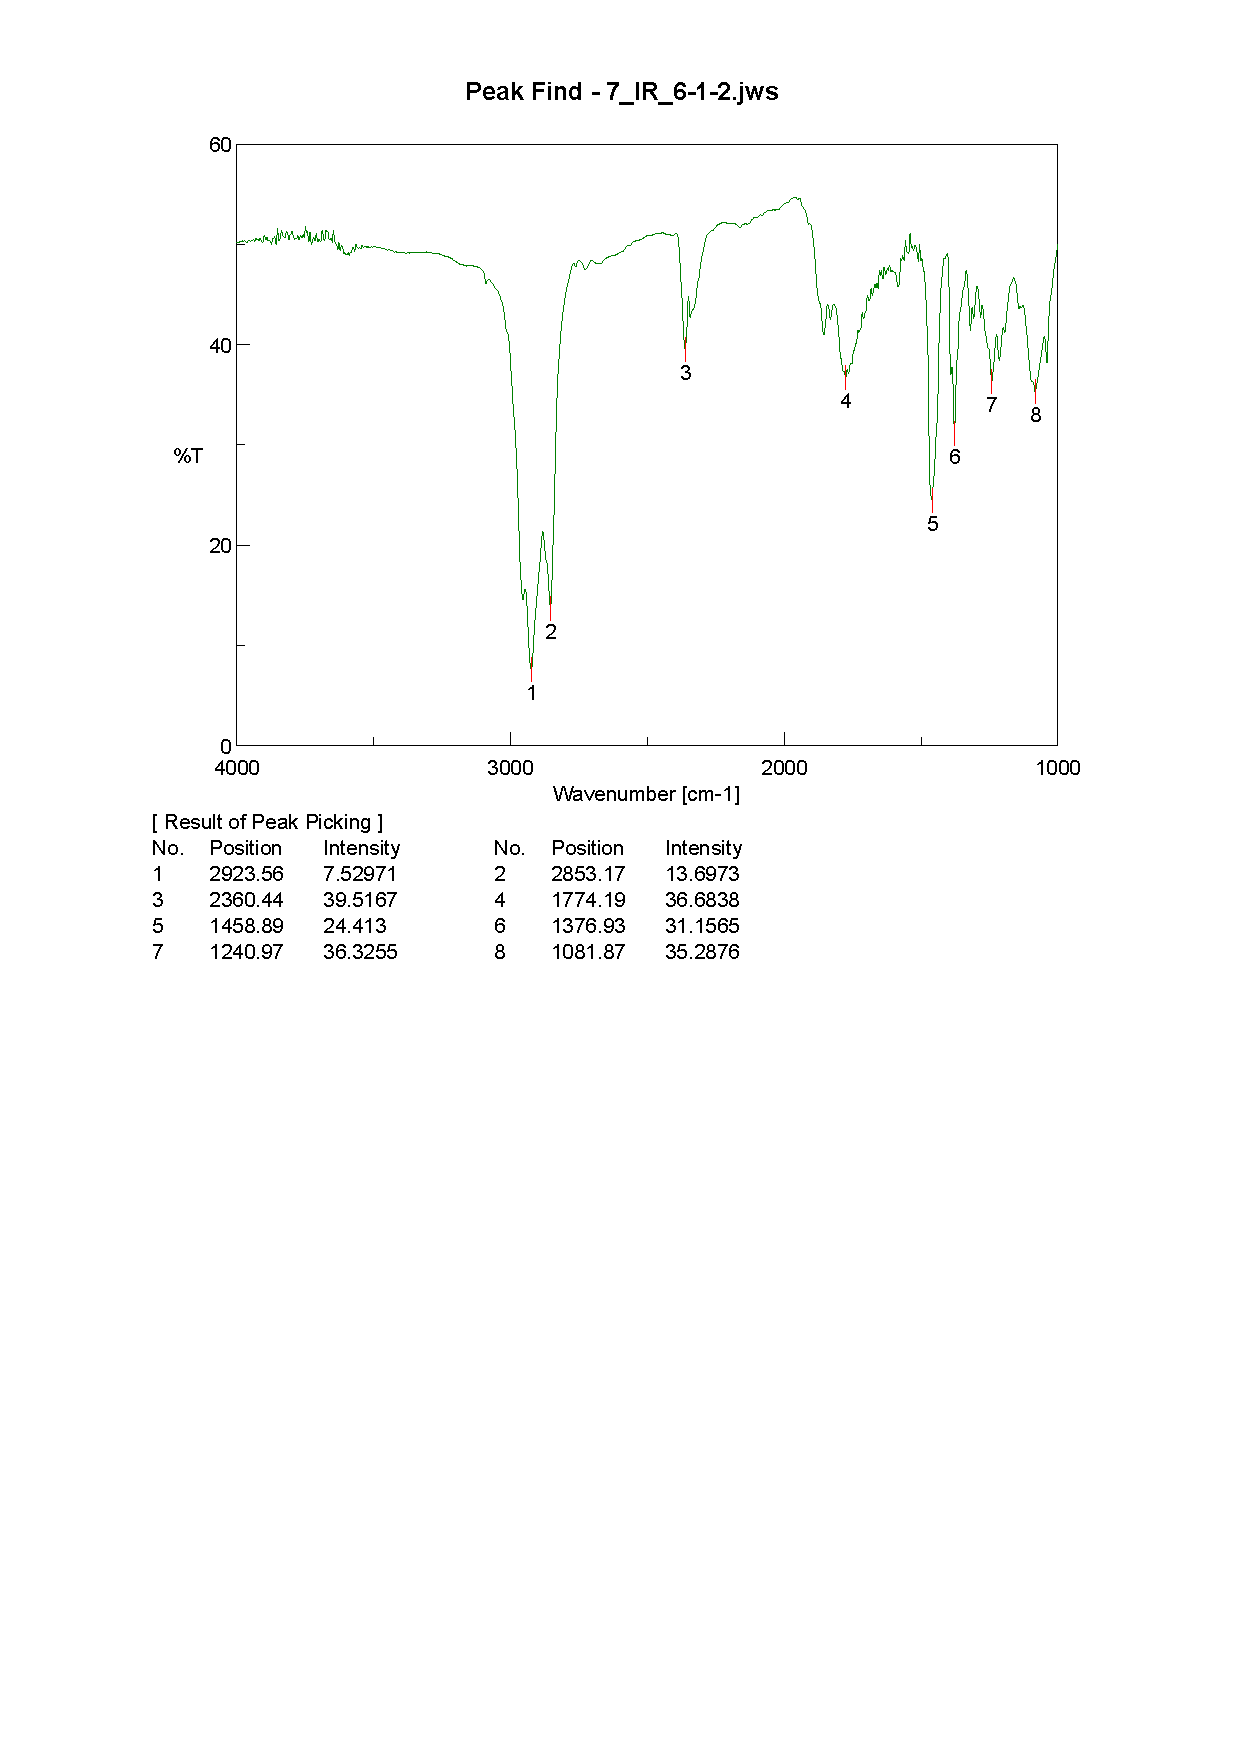
\includegraphics[width = 15 cm]{IR_6-1-2.pdf}
\caption{IR: \textbf{3} (nujol)}
\label{IR_6-1-2}
\end{center}
\end{figure}

\begin{figure}[htbp]
\begin{center}
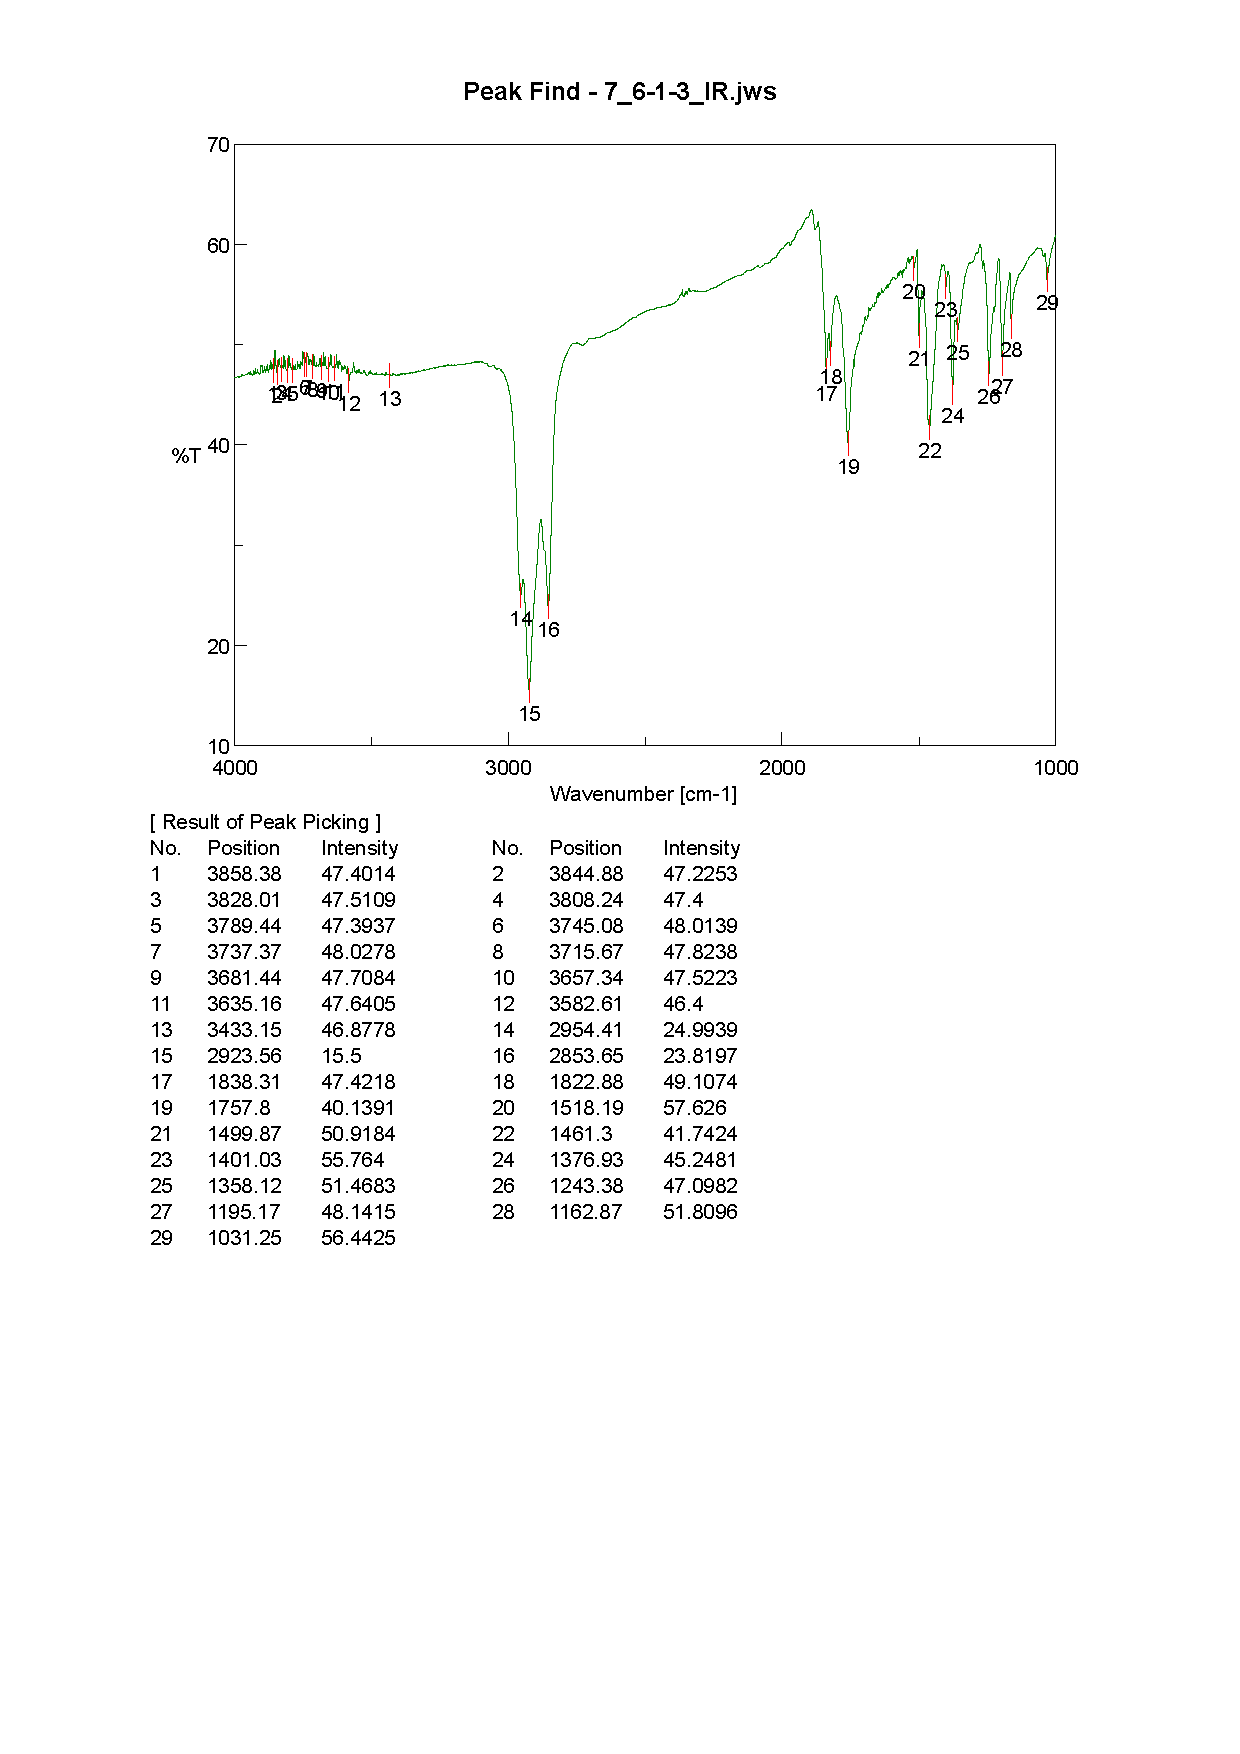
\includegraphics[width = 15 cm]{IR_6-1-3.pdf}
\caption{IR: \textbf{4} (nujol)}
\label{IR_6-1-3}
\end{center}
\end{figure}

\begin{figure}[htbp]
\begin{center}
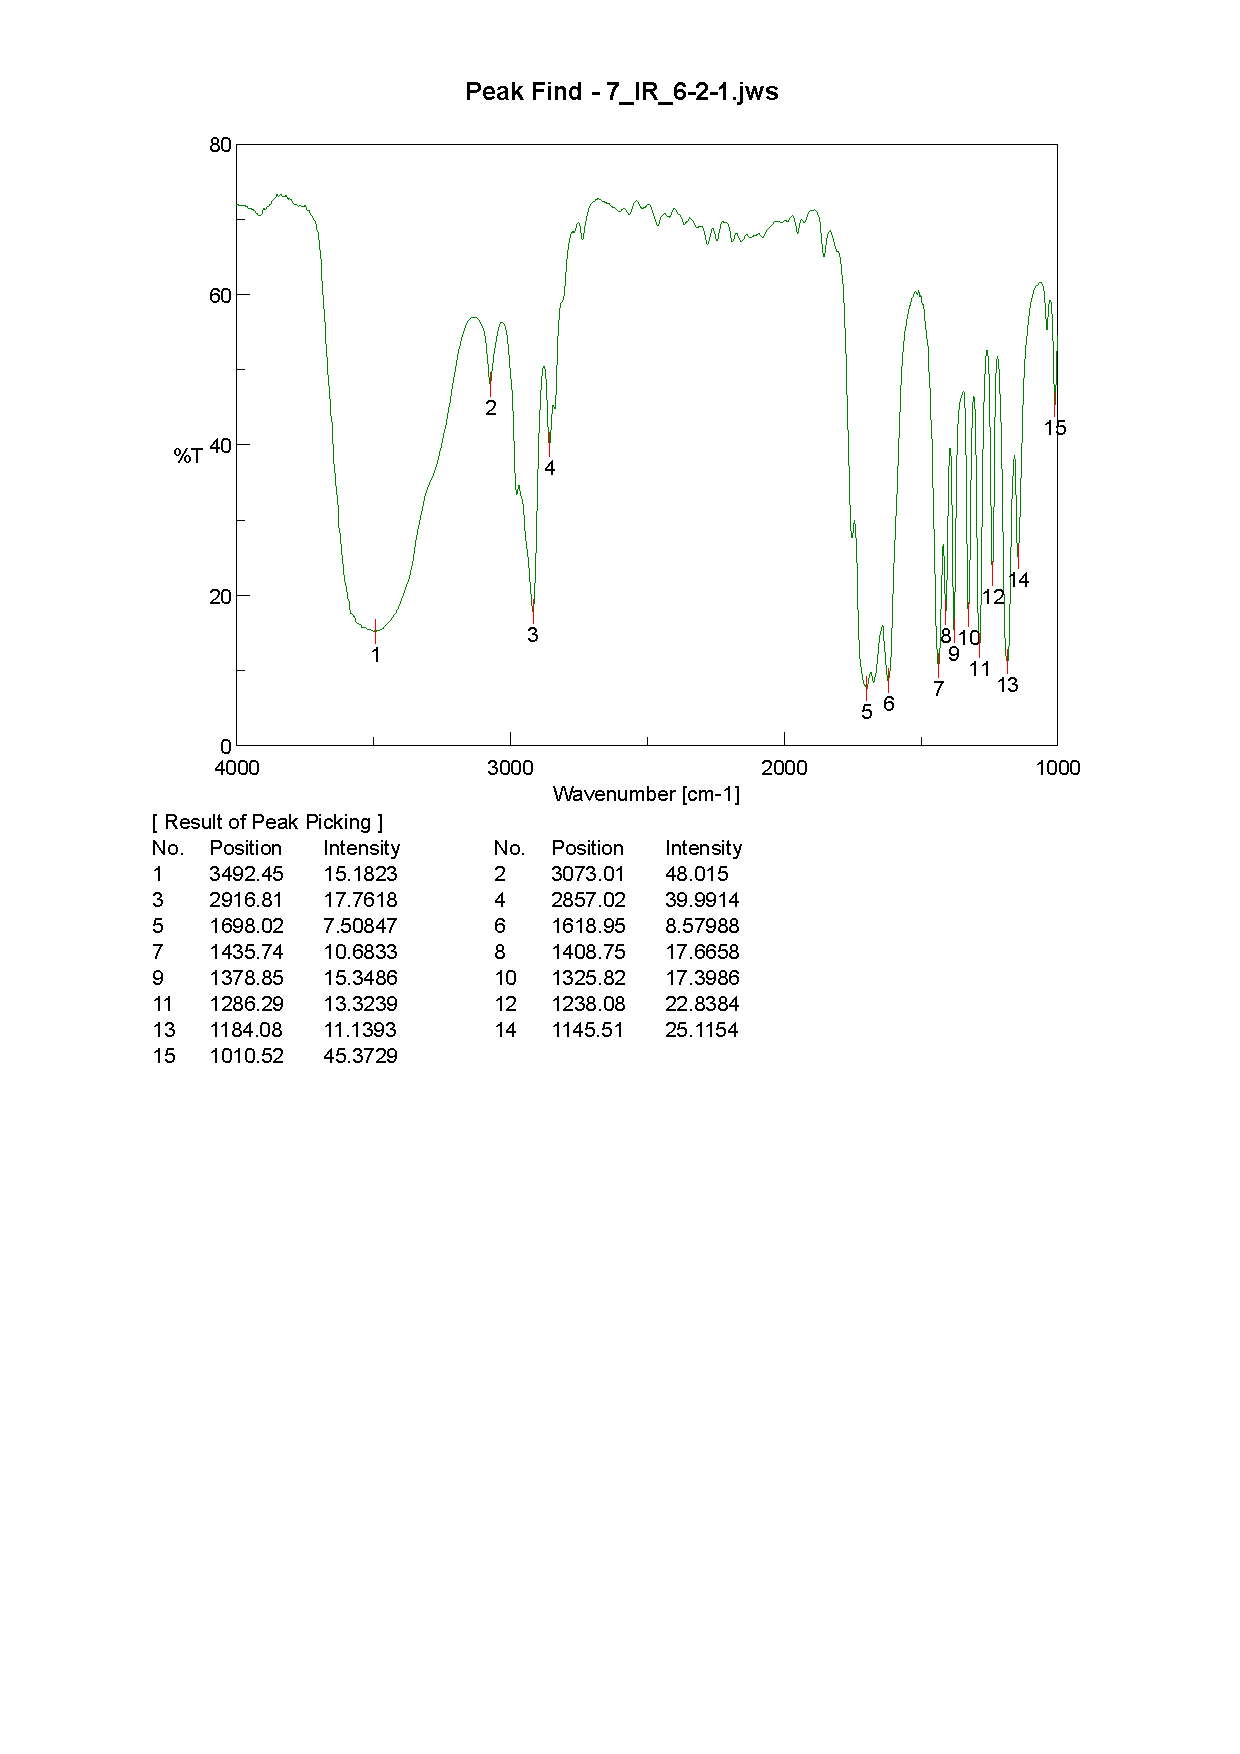
\includegraphics[width = 15 cm]{IR_6-2-1.pdf}
\caption{IR: \textbf{5}}
\label{IR_6-2-1}
\end{center}
\end{figure}


\begin{figure}[htbp]
\begin{center}
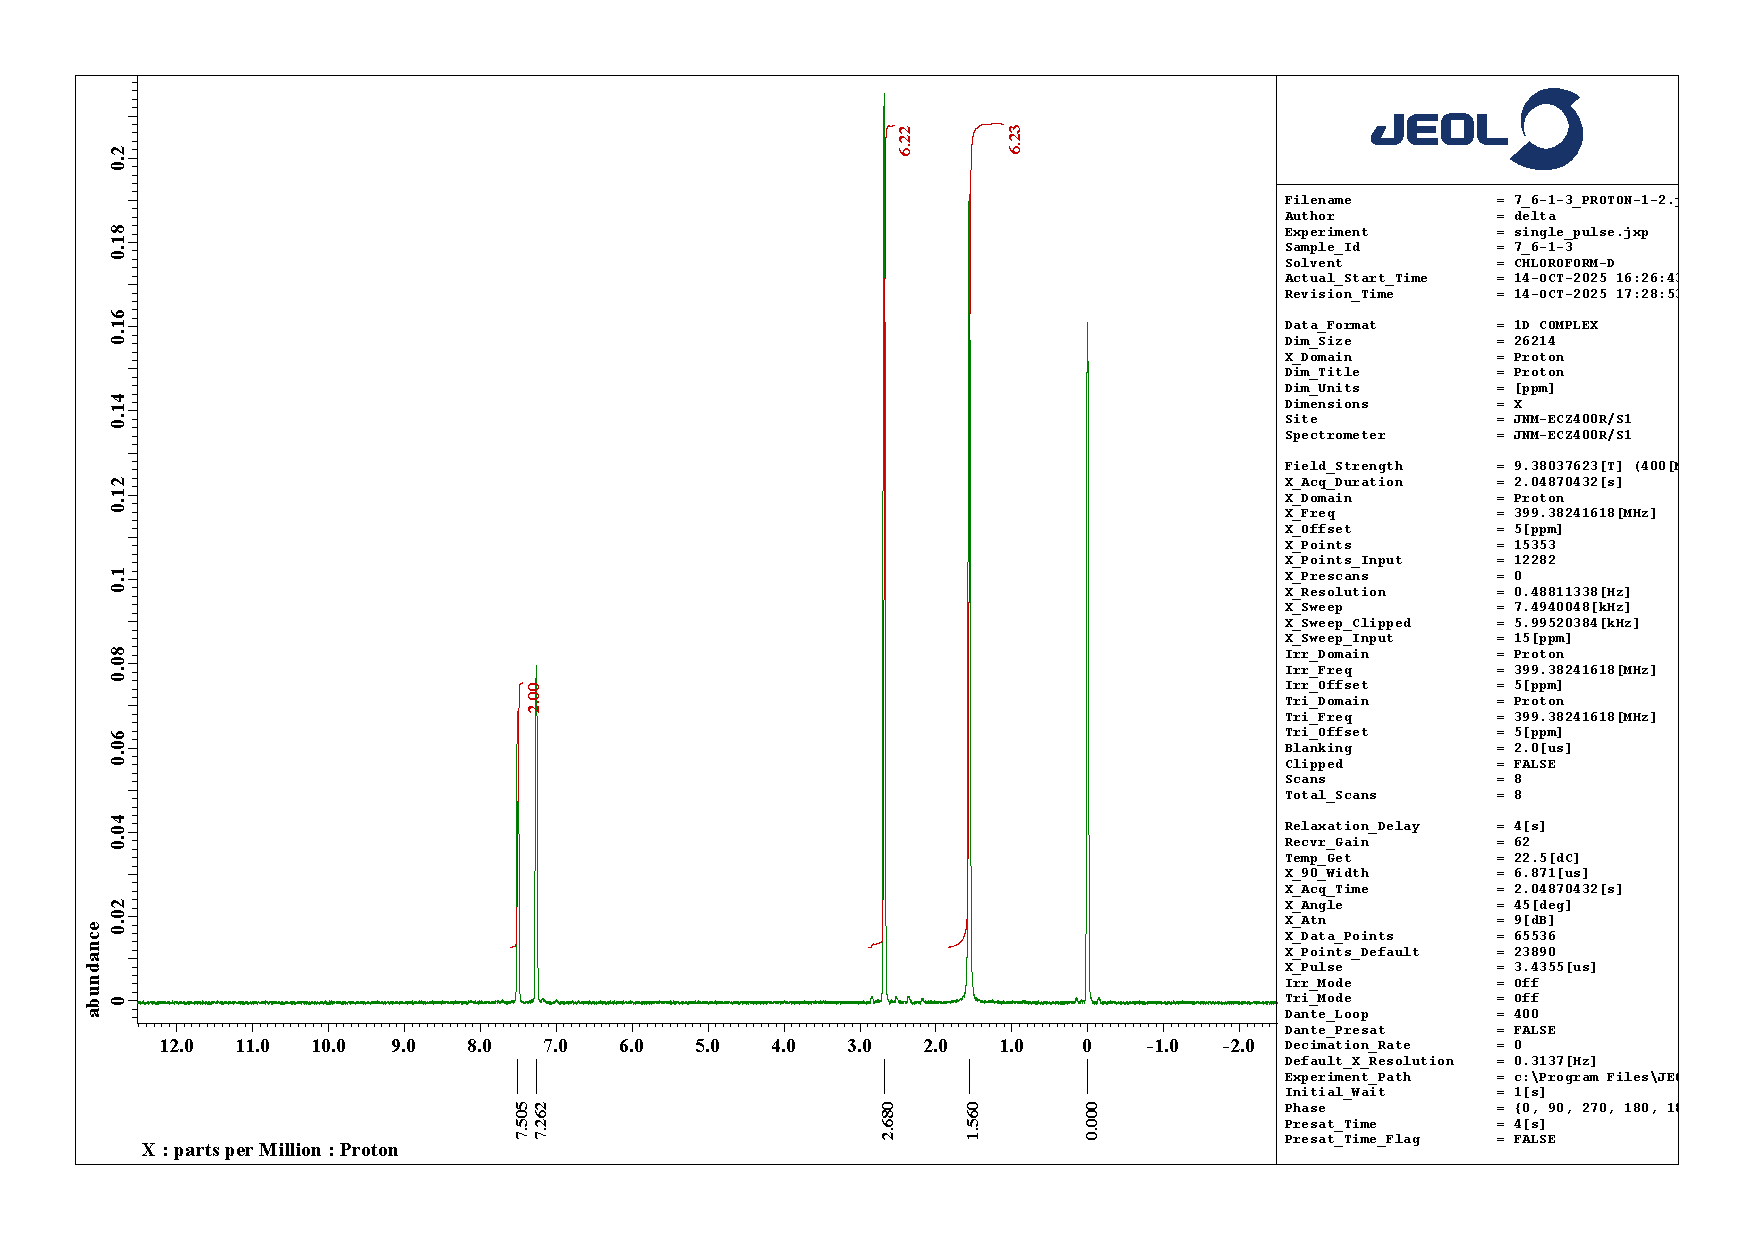
\includegraphics[width = 15 cm]{NMR_6-1-3.pdf}
\caption{NMR: \textbf{4} (溶媒: \ce{CDCl3})}
\label{NMR_6-1-3}
\end{center}
\end{figure}


\begin{figure}[htbp]
\begin{center}
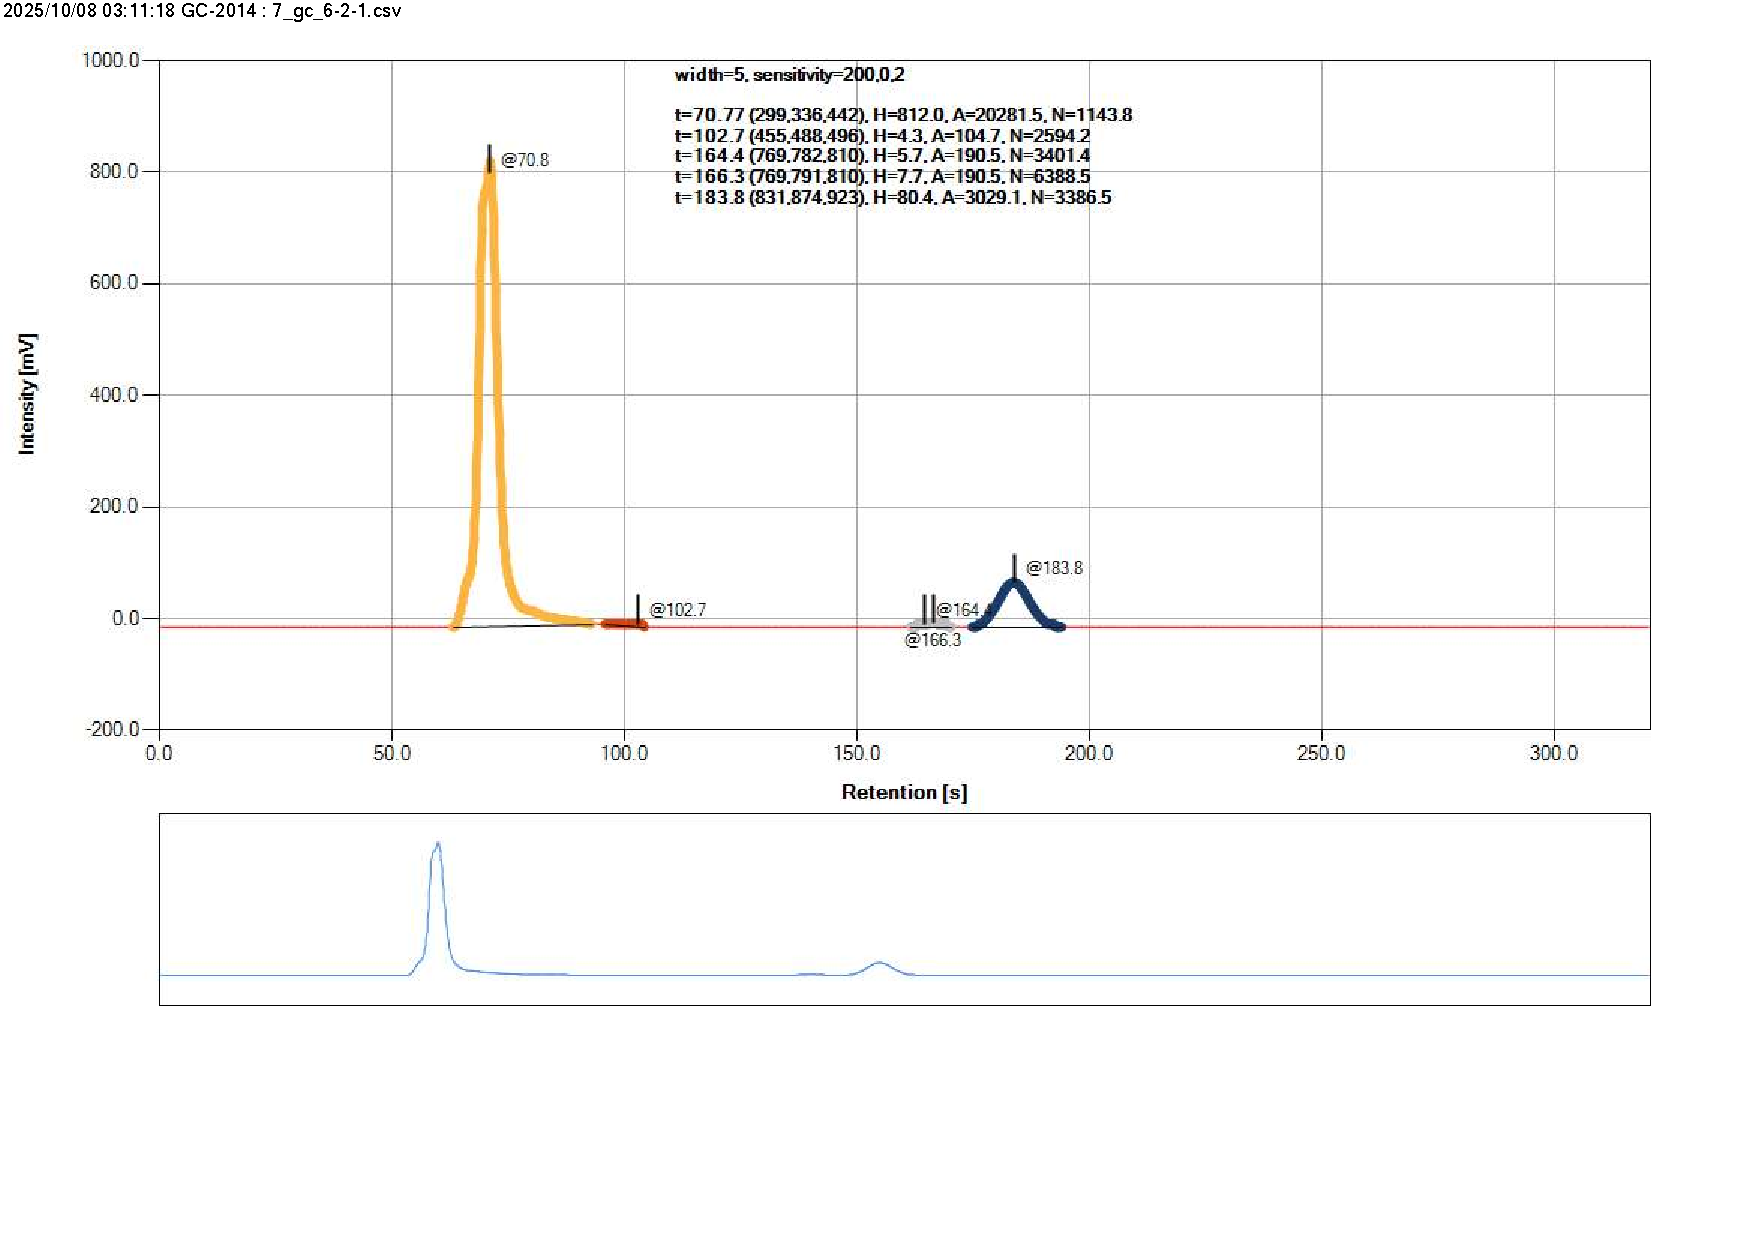
\includegraphics[width = 15 cm]{GC_6-2-1.pdf}
\caption{GC}
\label{GC_6-2}
\end{center}
\end{figure}


\begin{figure}[htbp]
\begin{center}
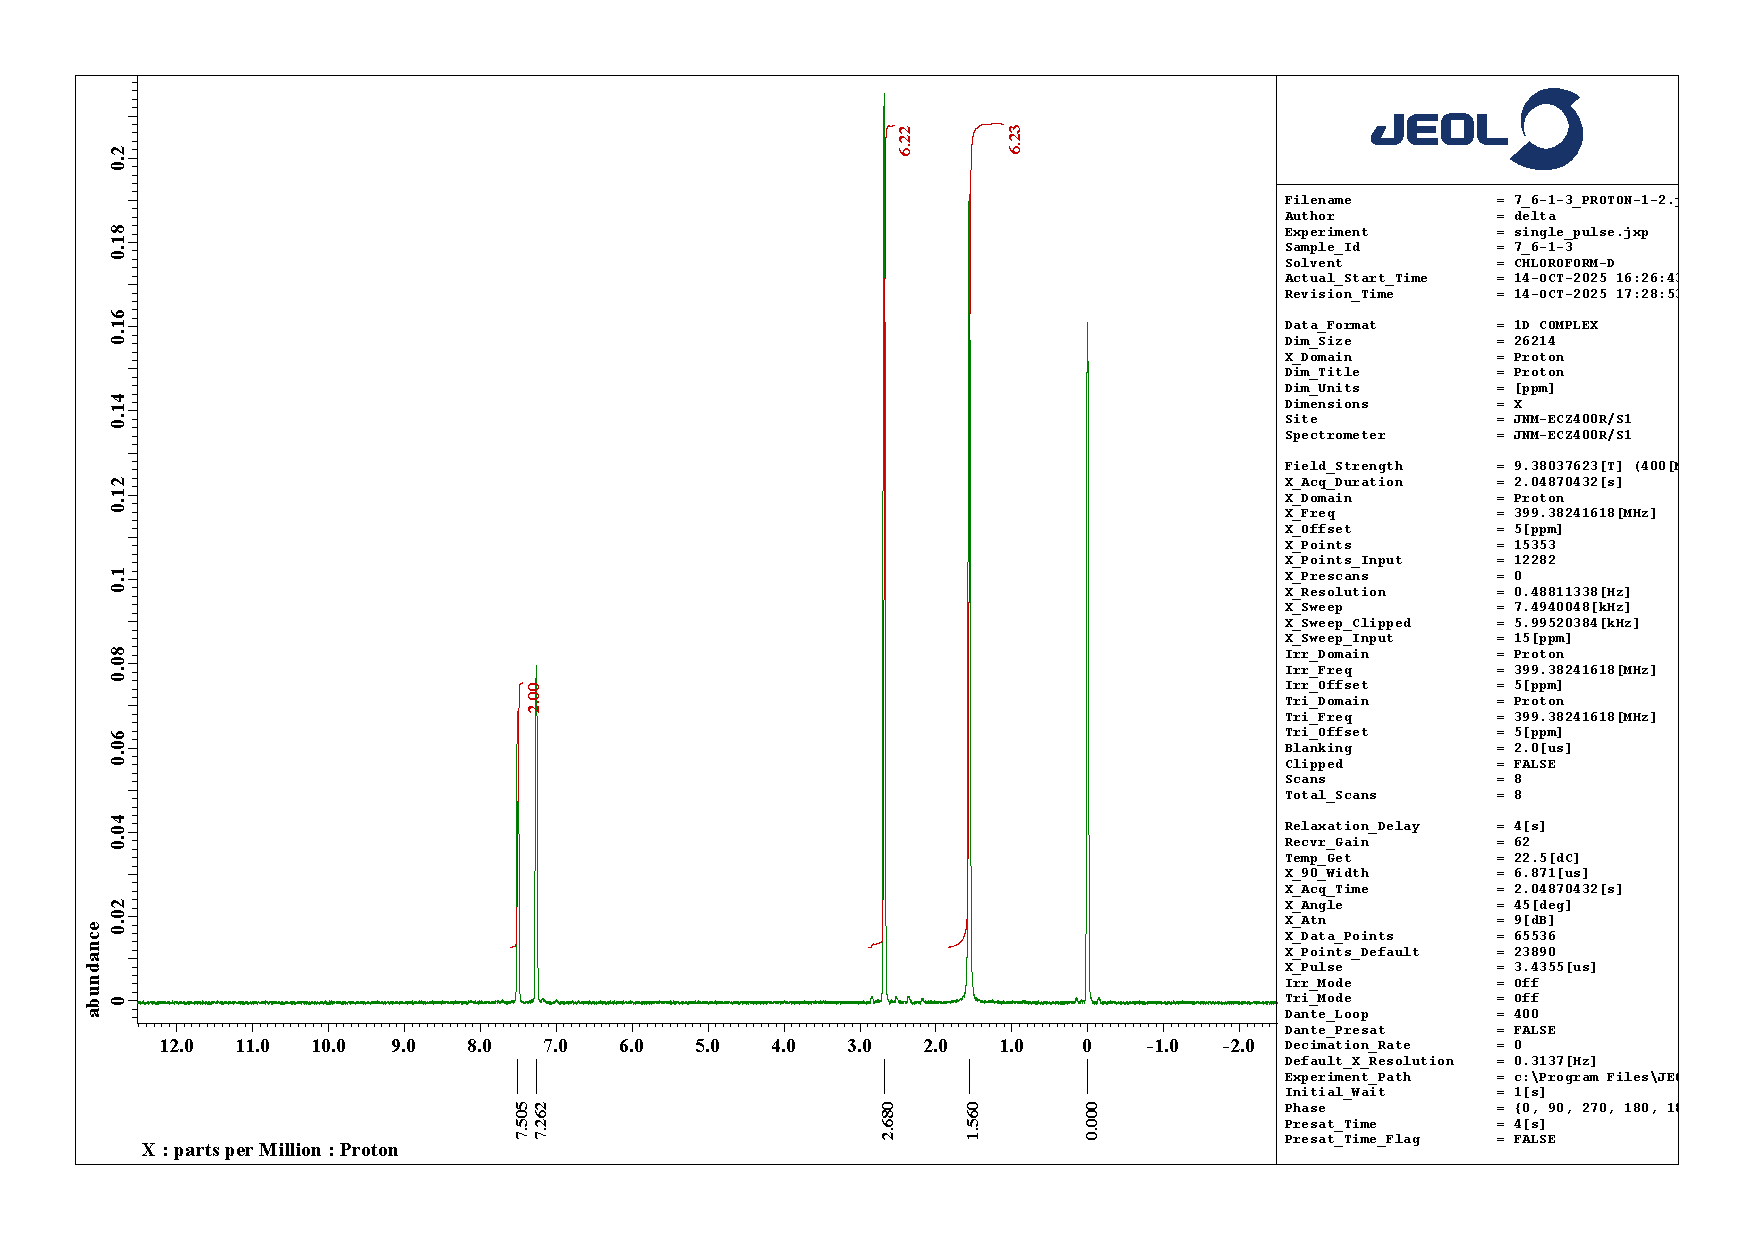
\includegraphics[width = 15 cm]{NMR_6-1-3.pdf}
\caption{NMR: \textbf{4} (溶媒: \ce{CDCl3})}
\label{NMR_6-1-3}
\end{center}
\end{figure}


\begin{figure}[htbp]
\begin{center}
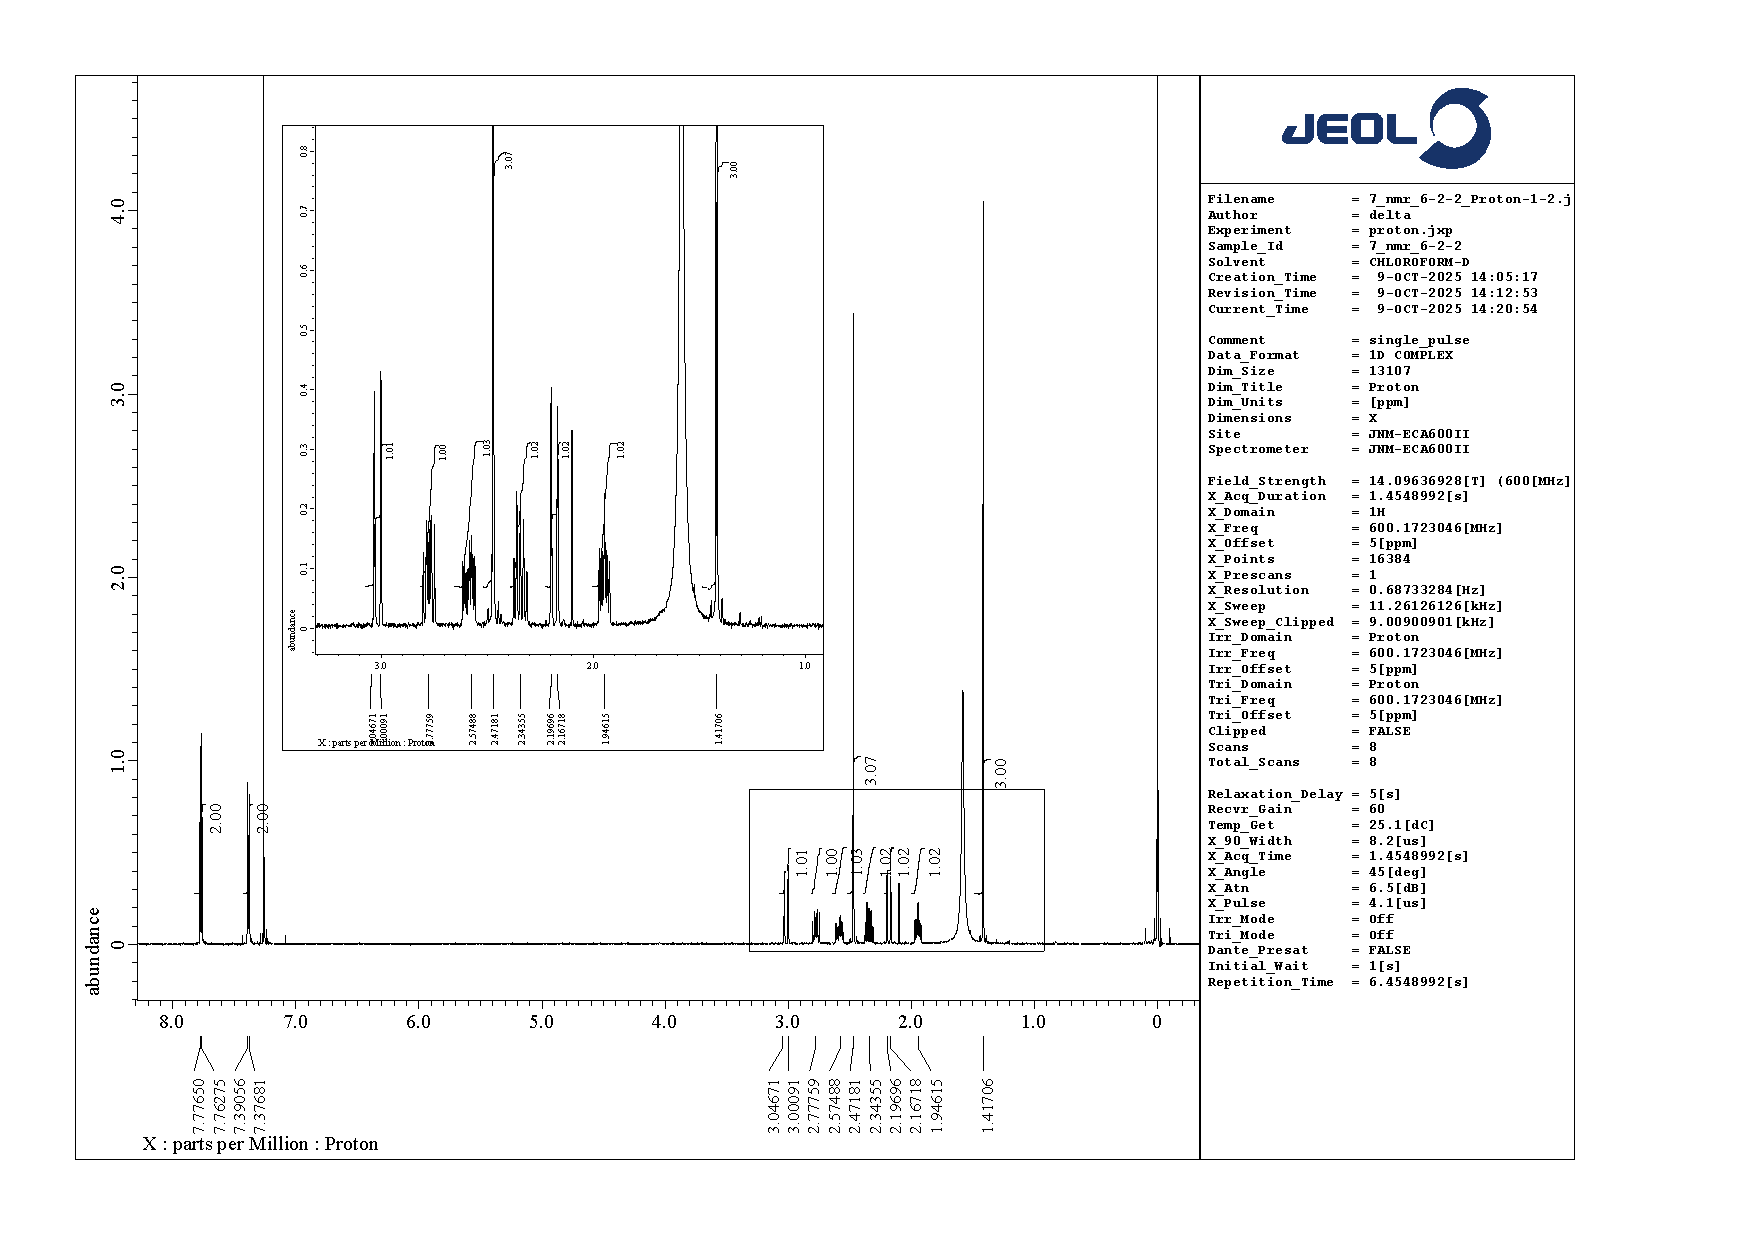
\includegraphics[width = 15 cm]{NMR_6-2-2.pdf}
\caption{NMR: \textbf{6} (溶媒: \ce{CDCl3})}
\label{NMR: 6-2-2}
\end{center}
\end{figure}

%%参考文献
\begin{thebibliography}{99}
\bibitem{nmr_solvent}
Hugo E. Gottlieb, Vadim Kotlyar, and
Abraham Nudelman, 
NMR Chemical Shifts of Common
Laboratory Solvents as Trace Impurities
J. Org. Chem. 1997, 62, 7512-7515
\bibitem{solvent_bp}
\url{https://www.tcichemicals.com/assets/cms-pdfs/organic-solvents-j.pdf}
\end{thebibliography}

\end{document}